% Preamble
% Document type
\documentclass{article}

% Additional packages
\usepackage[utf8]{inputenc}
\usepackage{wrapfig}
% Clickable Links in TOC
\usepackage[hidelinks]{hyperref}

% Images/ figures package
\usepackage{graphicx}
\graphicspath{ {./images/} }

% Language
\usepackage[ngerman]{babel}

% Information
\title{Projekt DeskPlanner}
\author{
Gökcek, Pinar\\
\texttt{pigoit00@hs-esslingen.de}
\and
Mezger, Kyle\\
\texttt{kymeit00@hs-esslingen.de}
\and
Imort, Jay\\
\texttt{jaimit00@hs-esslingen.de}
\and
Hofmann, Rico\\
\texttt{rihoit00@hs-esslingen.de}
\and
Pachtsinis, Darios\\
\texttt{dapait03@hs-esslingen.de}
}
\date{04. April 2022}

% Content
% Beginning of document
\begin{document}

% Titlepage
\begin{titlepage}
    \centering
    % Output title
    \maketitle

    % Hide page number
    \thispagestyle{empty}

    % Fill rest of page
    \vfill

\end{titlepage}

% Table of contents
\tableofcontents

\pagebreak

% \include{./tex_files/}
\chapter*{Zeitplan}


\begin{sidewaysfigure}[!ht]
    \centering
    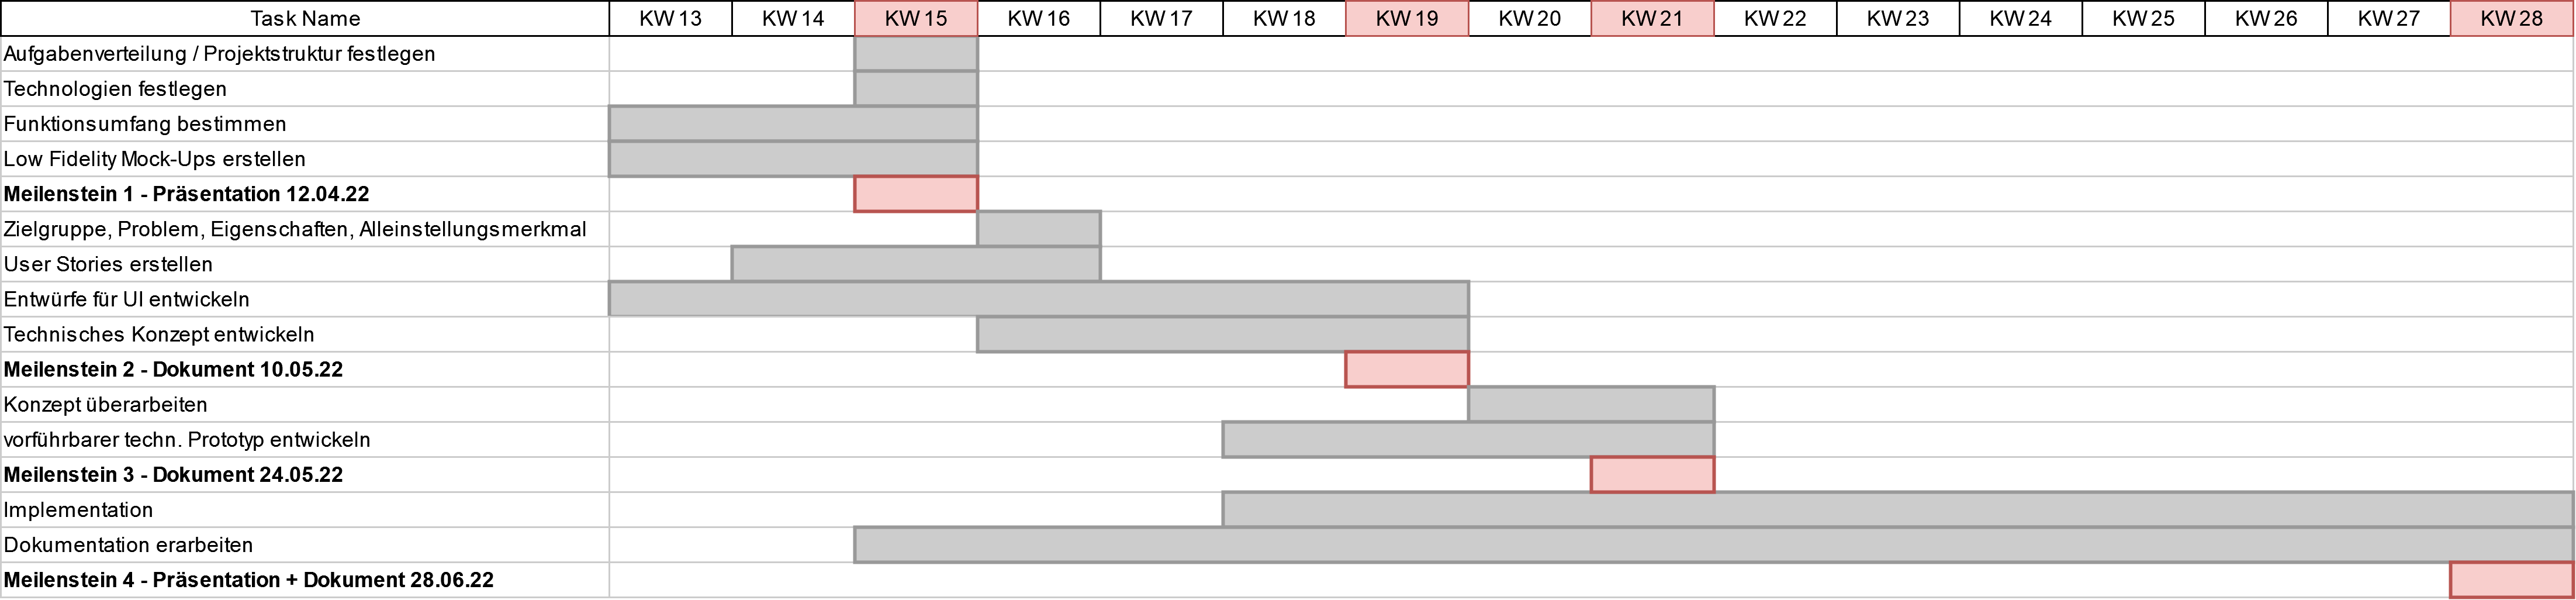
\includegraphics[width=0.6\textwidth]{Zeitplan_DeskPlanner.png}
    \caption{Zeitplan}
    \label{fig:Zeitplan}
\end{sidewaysfigure}

Der Zeitplan hangelt sich an den vorgegebenen Meilensteinen 1-4 entlang.
\\
\\
\textbf{Meilenstein 1 (12.04.22)}\\
Präsentation:
\begin{itemize}
    \item Aufgabenverteilung
    \item Projektmanagement
    \item Technologien
    \item Funktionsumfang
    \item UI-Entwürfe, z.B. Low Fidelity Mock-Ups
\end{itemize}

\vspace{0.03\textwidth}
\textbf{Meilenstein 2 (10.05.22)} \\
Dokumentation:
\begin{enumerate}
    \item Zielgruppe, Problem, Eigenschaften, Alleinstellungsmerkmal
    \item User Stories
    \item User Interface Entwürfe
    \item Technisches Konzept
    \begin{itemize}
        \item Verwendete Frameworks
        \item Softwarearchitektur
        \begin{itemize}
            \item UML-Verteilungsdiagramm des Gesamtsystems
            \item UML-Komponentendiagramm (jeweils für Client und Server)
        \end{itemize}
        \item Datenbank
        \begin{itemize}
            \item Entity Relationship Model
        \end{itemize}
    \end{itemize}
    \item UI-Entwürfe, z.B. Low Fidelity Mock-Ups
\end{enumerate}

\textbf{Meilenstein 3 (24.05.22)}

\textbf{Meilenstein 4 (28.06.22)}

\section{Zielgruppe, Problem, Eigenschaften, Alleinstellungsmerkmal}

\subsection{Zielgruppe}

Aufgrund der Coronapandemie wurden Konzepte wie Home-Office in vielen Industrien ausprobiert, in denen es so etwas zuvor wenig gab.
Mit diesen neuen Nutzern von dynamischen Arbeitsplatzkonzepten ist der potentielle Nutzerstamm für eine Anwendung zum dynamischen Zuweisen von Arbeitsplätzen stark gestiegen.
Maximal waren während der Pandemie in ein Umfrage der Hans-Böckler-Stiftung 27\% der Befragten im Home-Office.
Laut dem Ifo-Institut können ca 56\% aller Arbeitnehmer zumindest teilzeit im Home-Office Arbeiten. 
Das zeigt für wie viele Arbeitnehmer ein Dynamisches Arbeitsplatzkonzept wie unseres eine Möglichkeit wäre.

\begin{figure}[!h]
    \centering
    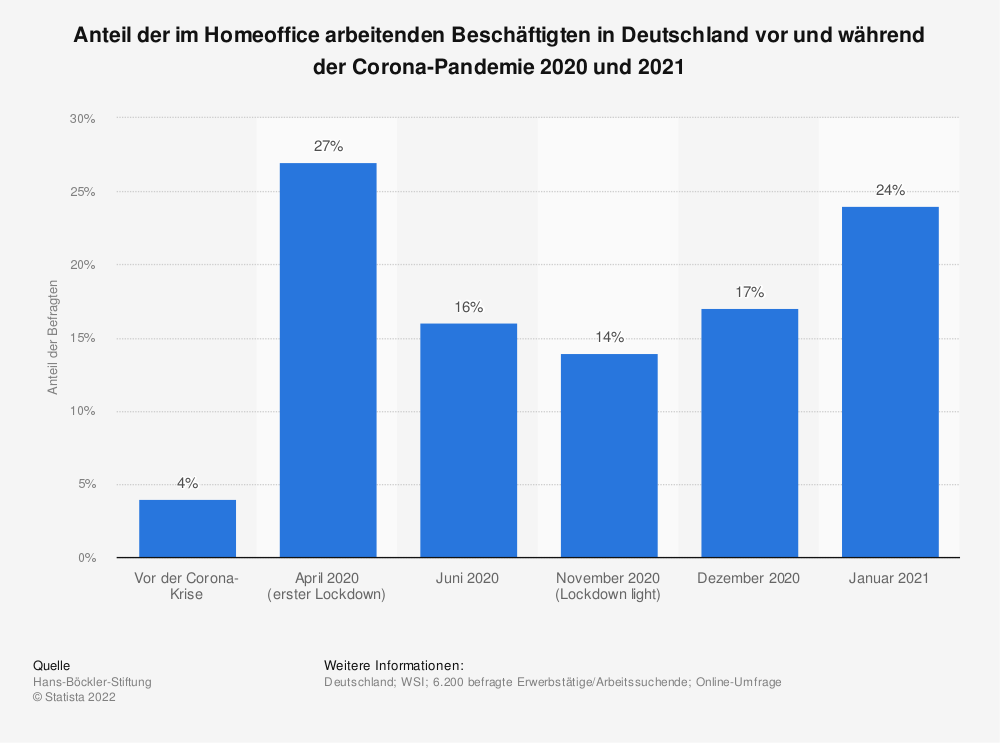
\includegraphics[width=0.8\textwidth]{statistik_homeoffice_corona.png}
    \caption{Home Office}
    \label{fig:HomeOffice}
\end{figure}

Dafür müssen aber auch Home-Office skeptische Arbeitgeber von den Vorteilen eines dynamischen Arbeitsplatzsystems, wie z.B. reduzierte Büro-Flächen und so geringere Miet- / Baukosten, überzeugt werden.
\pagebreak
\\
\textbf{Personas: }

\begin{figure}[!h]
    \centering
    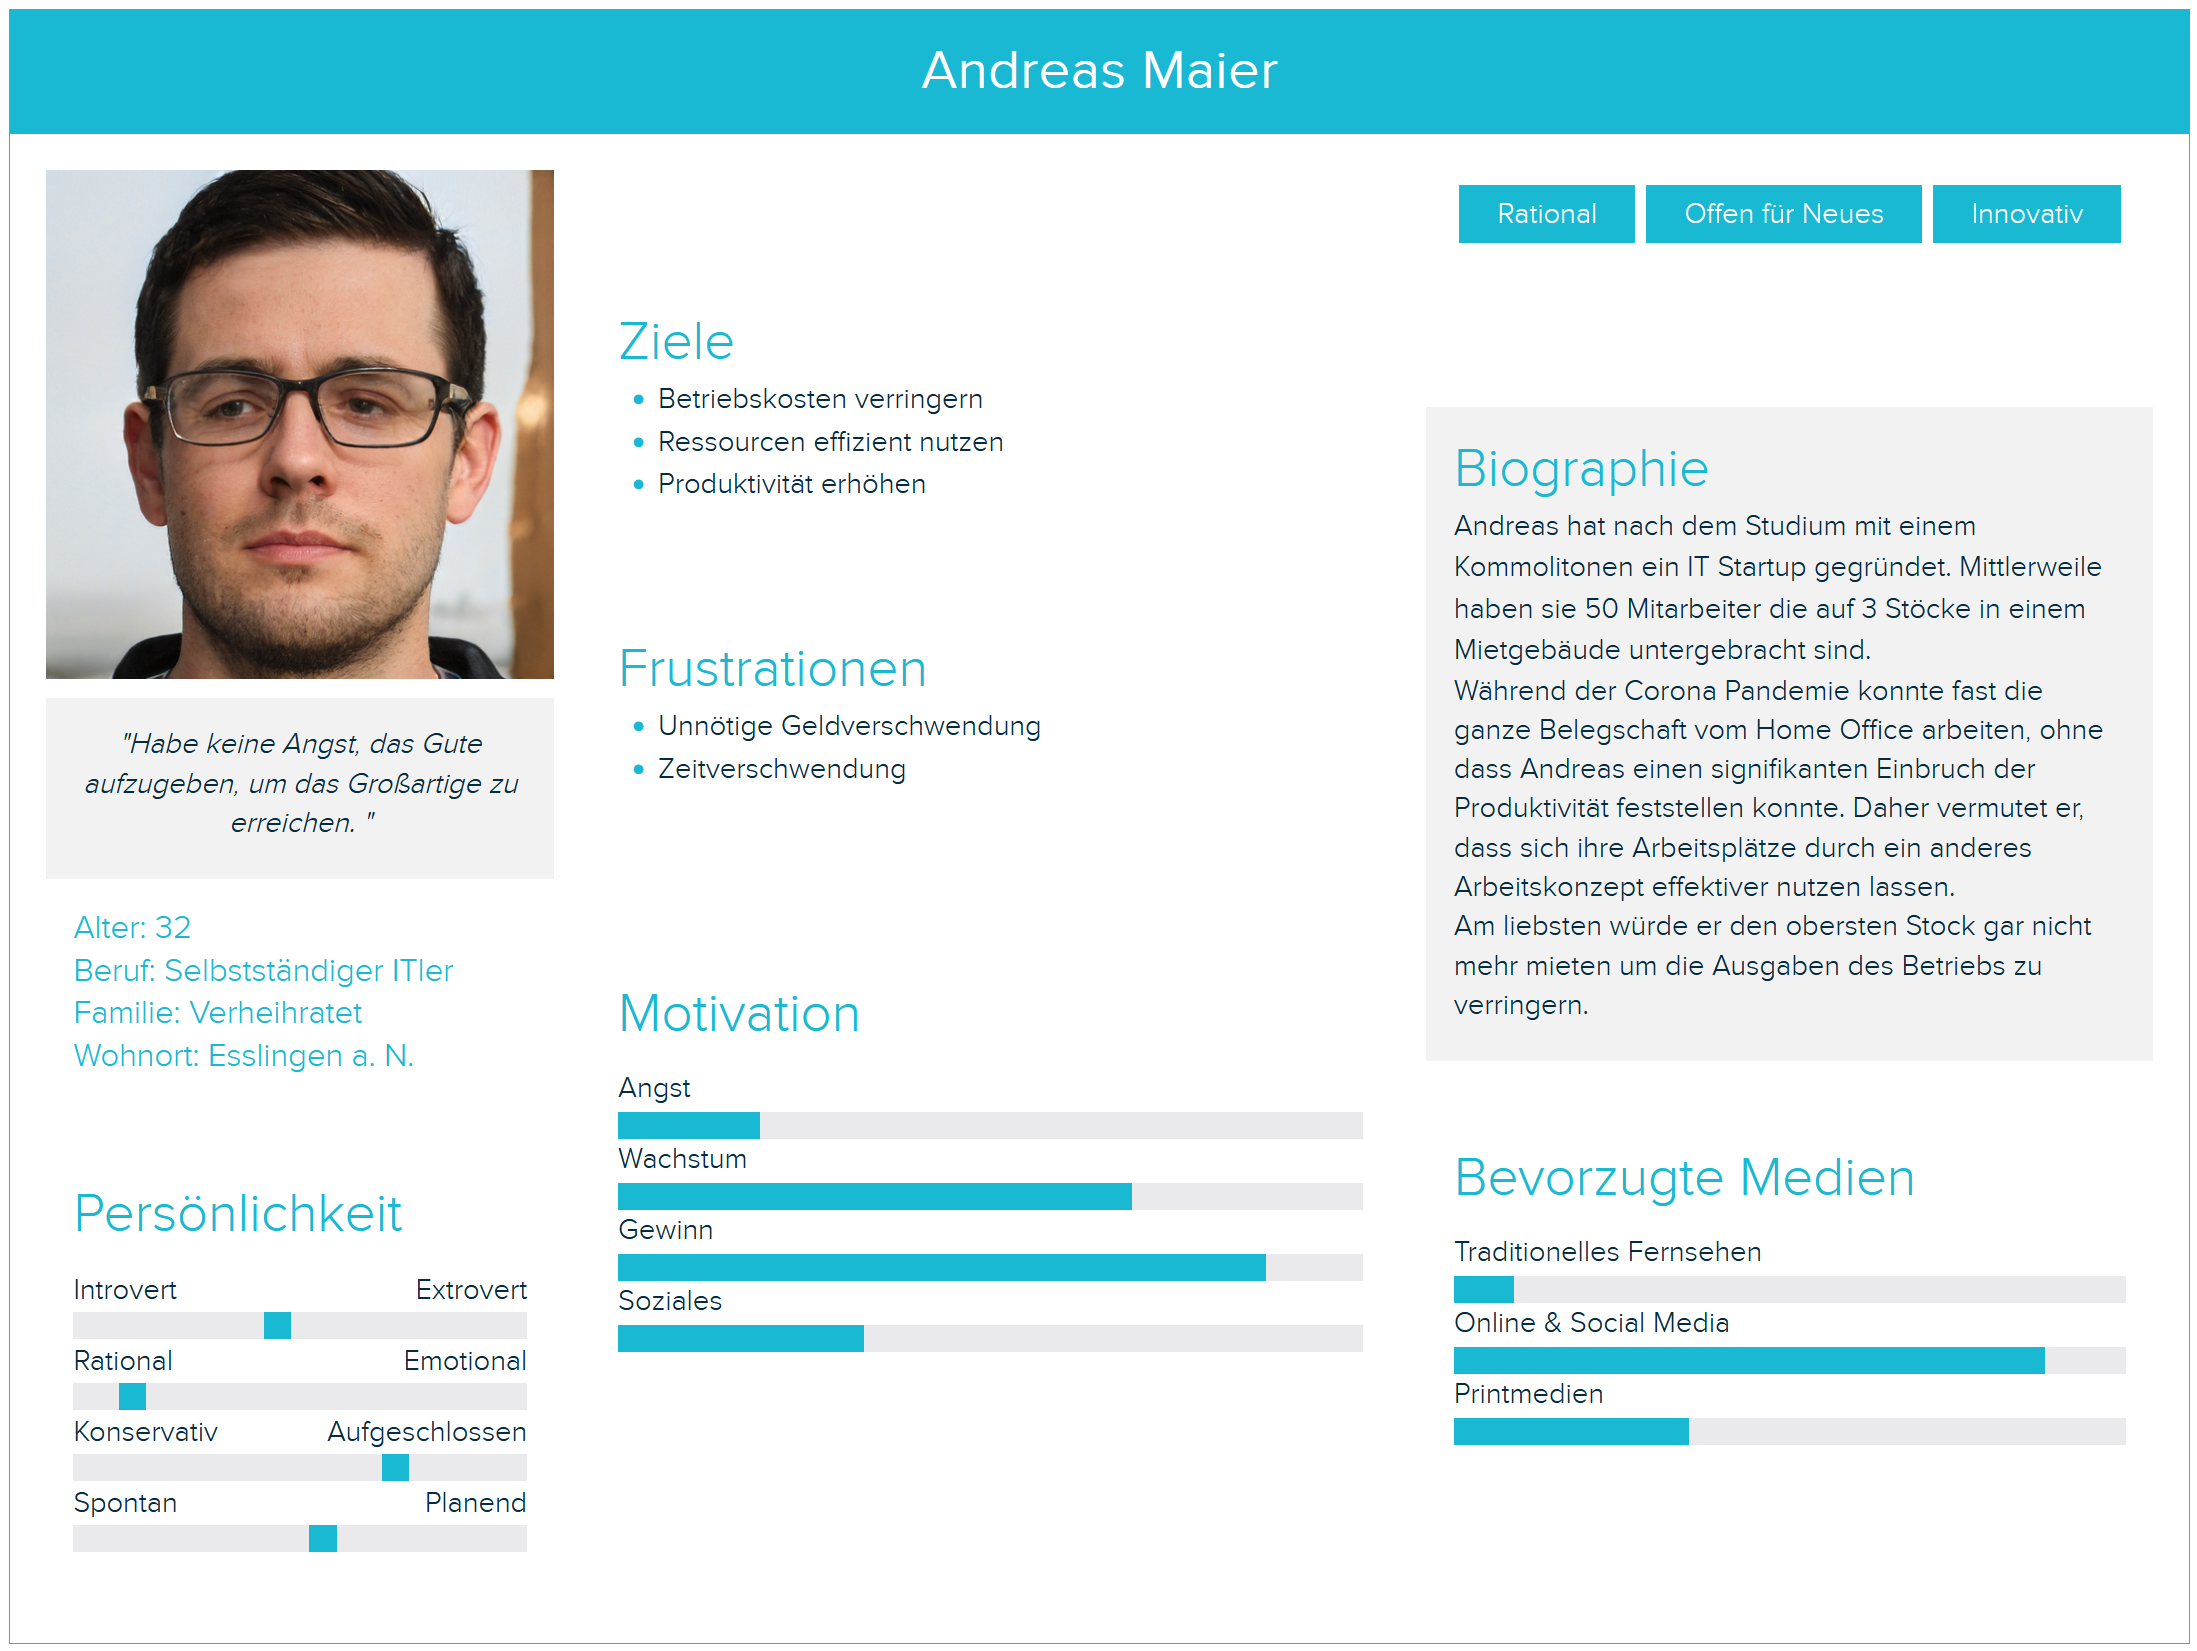
\includegraphics[width=1\textwidth]{Persona_Andreas_Maier.png}
    \caption{Persona Andreas Maier}
    \label{fig:PersonaAndreasMaier}
\end{figure}

Andreas repräsentiert den offensichtlichsten potentiellen Kunden.
Er erkennt selbst schon das Potential von nicht traditioneller Arbeitsplatznutzung und kommt schon von sich aus auf die Idee, nach den Erkenntnissen durch die Corona Zeit, die Arbeitsplatznutzung in seiner Firma umzustellen.\\
Er kann vermutlich mit rationalen Argumenten zur Kostenminderung, effizienten Zeitnutzung etc. von unserem Konzept überzeugt werden, hat aber auch hohe Ansprüche an Funktionalität und allgemeine Qualität der Anwendung.

\pagebreak

\begin{figure}[!h]
    \centering
    \includegraphics[width=1\textwidth]{Persona_Gerd_Ovelgönne.png}
    \caption{Persona Gerd Ovelgönne}
    \label{fig:PersonaGerdOvelgönne}
\end{figure}

Gerd ist Repräsentant einer konservativen Nutzergruppe, die noch nicht voll vom Konzept dynamischer Arbeitsplatzbelegung überzeugt sind, aber genug Motivationen haben, um potentiell von den Vorteilen überzeugt zu werden.
\\
Gerd ist schon sehr lange in seinem Beruf.
Er weiß genau was wie zu laufen hat und macht daher nur ungern Veränderungen.
\\
Durch die Vorgabe seiner Firma hat er jedoch eine externe Motivation, um das Arbeitskonzept seiner Abteilung zumindest ein wenig umzustellen.
Da Gerd zufriedene Mitarbeiter als Ziel hat, wäre das noch eine Motivation auf Umstellung, die wir in Werbung ansprechen könnten.
Den Mitarbeitern mehr Flexibilität zu bieten, sowohl in der reinen Wahl wo in der Abteilung sie sitzen als auch in der Entscheidung ob sie eine Arbeit von Zuhause erledigen können, kann sich positiv auf die Zufriedenheit der Mitarbeiter auswirken.
Vor allem wenn flexibleres Arbeiten durch die Vorgabe der Geschäftsführung in anderen Abteilungen möglich wird, sollten den eigenen Mitarbeitern auch ähnliche Möglichkeiten geboten werden um Frustration zu verhindern.
\\
Ihm sollten, da ihm Home-Office nicht so gefällt, auch Vorteile einer flexiblen Arbeitsplatznutzung ohne Home-Office gezeigt werden, wie bspw. die Einrichtung von Ruhearbeitszonen oder die Wahl der Arbeitsplätz entsprechend der Arbeit die an einem Tag stattfindet.


\subsection{Problem}
Während der Pandemiezeit wird verstärkt von Zuhause aus gearbeitet, dadurch schwankt die Anzahl der Arbeiter im Büro stark und die interdisziplinären Kollegen habe keinen Überblick mehr darüber, wer im Büro ist und wer nicht.
Zumal grundsätzlich nicht jeder in das Home-Office kann bzw. will, dies kann diverse Gründe, wie z. B. fehlende Räumlichkeiten oder die geschwächte Konzentrationsfähigkeit in den eigenen vier Wänden sein.
Agile Arbeitsplätze haben den Vorteil, dass der Arbeitsplatz je nach momentanem empfinden gewählt werden kann z. B. im sogenannten Ruhebereich, Bereiche die näher an Heizkörpern sind oder hellere Arbeitsplätze an Fenstern.
Projektspezifisch kann es vorteilhaft sein neben einem bestimmten Kollegen zu arbeiten, um den Austausch produktiver zu gestalten.
Diese Bereiche können frei benutzt werden, sofern diese nicht durch eine andere Kollegin oder einen anderen Kollegen belegt sind.
Derzeit ist es gängig, dass die Bereiche nach dem Prinzip “first come first serve“ besetzt werden. 

\paragraph{} Wenn man am Morgen an einem Arbeitsplatz sitzt, dann aber im Laufe des Tages für einen längeren Zeitraum diesen verlassen muss, wird diese Ressource unnötig blockiert.
Raumbelüftungssysteme, Heizungen und Klimaanlagen für Räume bzw. Gebäude werden nicht nach der Personenauslastung betrieben, in Hinblick auf die steigenden Energiekosten, ist dies weder ökonomisch noch nachhaltig.
Immungeschwächte Personen die ihre Tätigkeit nur vor Ort im Büro erledigen können, haben pandemiebedingt nicht die Möglichkeit Arbeitsplätze zu Buchen, die weiter weg von den restlichen Arbeitsplätzen bzw. Kollegen sind. 
Der Arbeitgeber, der nur eine bestimmte X Arbeitsplätzen hat, kann nicht mehr als X Arbeiter in dem Bürokomplex beschäftigen. 
Desweitern gibt es derzeit keine einfache Möglichkeit die Büro Belegschaft, über einen längeren Zeitraum zu analysieren. 
Diese Analyse kann unter anderem zur dauerhaften Arbeitsplatz Reduktion, bei gleicher Mitarbeiterzahl führen.

\paragraph{} Unsere Anwendung ermöglicht es, die oben angesprochenen Fälle zu Gunsten des Arbeitgebers und -nehmers zu lösen.
Die Raumplanung ermöglichet eine Buchung in 15 min Rastern auch Dauerbuchungen über mehrere Monate sind möglich.
Nicht nur Arbeitsplätze in einem Raum, sondern bestimmte Räume in bestimmten Gebäuden können gebucht werden.
Auch ist eine Chatfunktion zwischen Teamleitern und Mitarbeitern bzw. zwischen Mitarbeitern möglich.
Dies hat den Vorteil das Buchungen bei Sonderfällen unter Mitarbeitern einfach getauscht werden können.
Eine Synchronisation mit dem Outlookkalender wäre auch denkbar.

\subsection{Eigenschaften}
Die Web-Applikation DeskPlanner wird mindestens folgende Eigenschaften \\nachweisen können:

\begin{itemize}
    \item Open Source (Lizenzfrei) als kostenfreie Möglichkeit für vor allem kleine Unternehmen
    \item Simple Möglichkeiten, um Komplexität zu vermeiden, aber so viele Mög-lichkeiten der Raumplanung beizubehalten
    \item Three-Tier Architecture ähnliche Anwendungsweise der Raumplanung im Sinne von Gebäude > Stockwerk > Raum 
\end{itemize}

\paragraph{} Des Weiteren sind kleine Eigenschaften wie Einhaltung der 7 Usability Prinzipien vorgesehen, um so die Bedienung des Kunden so einfach wie möglich zu halten. 
Beispiele hierfür sind Hilfstexte, welche die verschiedenen Buttons erklären sollen oder selbsterklärende Icons der jeweiligen Buttons. 
Außerdem soll der Nutzer nicht mit Information beschüttet werden, sondern eine auf seinen Nutzungskontext angepasste Benutzeroberfläche sorgen für Aufgabenangemessenheit. 
Durch die individuelle Raumgestaltung erhält der Nutzer ein steuerbares Softwaresystem, welches genau das machen wird, was der Nutzer auch erwartet.

\subsection{Alleinstellungsmerkmal}
Als herausragendes Leistungsmerkmal des DeskPlanners bezeichnet man die effiziente Arbeitsplatznutzung. 
In der heutigen Branche, vor allem durch Corona bestätigt, gilt es, die Kosten immer weiter zu reduzieren. 
Durch die Raumbuchungsmöglichkeiten, kann ein Unternehmen die Arbeitsplätze minimieren, Home Office Mitarbeiter perfekt einplanen und dadurch Kosten der Technik und Größe des Raumes einsparen für andere Investitionen. 
Als Open Source Web-Applikation kann ein Unternehmen sogar lizenzfrei den Arbeitsplatz kosteneffizienter nutzen.
Genau hier soll der DeskPlanner vor allem kleineren Unternehmen unterstützen, um auch in Zeiten der Pandemie nicht insolvent zu gehen.


<<<<<<< HEAD
\subsection{Problem}
Während der Pandemiezeit wird verstärkt von Zuhause aus gearbeitet, dadurch schwankt die Anzahl der Arbeiter im Büro
stark und die interdisziplinären Kollegen habe keinen Überblick mehr darüber, wer im Büro ist und wer nicht.
Auch die Geschäftsleitung hat keine direkte Möglichkeit, ohne die entsprechenden Teamleiter zu kontaktieren, sich über 
die Momentane Anwesenheit zu informieren.
Zumal grundsätzlich nicht jeder in das Home-Office kann bzw. will, dies kann diverse Gründe, wie z. B. fehlende
Räumlichkeiten oder die geschwächte Konzentrationsfähigkeit in den eigenen vier Wänden sein. Agile Arbeitsplätze
haben den Vorteil, dass der Arbeitsplatz je nach momentanem empfinden gewählt werden kann z. B. im sogenannten Ruhebereich,
Bereiche die näher an Heizkörpern sind oder hellere Arbeitsplätze an Fenstern. Projektspezifisch kann es vorteilhaft sein
neben einem bestimmten Kollegen zu arbeiten, um den Austausch produktiver zu gestalten. Diese Bereiche können frei benutzt werden,
sofern diese nicht durch eine andere Kollegin oder einen anderen Kollegen belegt sind. Derzeit ist es gängig, dass die Bereiche nach
dem Prinzip “first come first serve“ besetzt werden.\\\\
Wenn man am Morgen an einem Arbeitsplatz sitzt, dann aber im Laufe des Tages für einen längeren Zeitraum diesen verlassen muss,
wird diese Ressource unnötig blockiert. Raumbelüftungssysteme, Heizungen und Klimaanlagen für Räume bzw. Gebäude werden nicht
nach der Personenauslastung betrieben, in Hinblick auf die steigenden Energiekosten, ist dies weder ökonomisch noch nachhaltig.
Theortisch ist es auch möglich durch die hierdurch gewonnene Statistik, die Raum- bzw. Gebäudeausnutzungen zu optimieren
und dadurch Mietkosten einzusparen.
Immungeschwächte Personen die ihre Tätigkeit nur vor Ort im Büro erledigen können, haben pandemiebedingt nicht die Möglichkeit
Arbeitsplätze zu Buchen, die weiter weg von den restlichen Arbeitsplätzen bzw. Kollegen sind. Der Arbeitgeber, der nur eine bestimmte
X Arbeitsplätzen hat, kann nicht mehr als X Arbeiter in dem Bürokomplex beschäftigen. Desweitern gibt es derzeit keine einfache Möglichkeit
die Büro Belegschaft, über einen längeren Zeitraum zu analysieren. Diese Analyse kann unter anderem zur dauerhaften Arbeitsplatz Reduktion,
bei gleicher Mitarbeiterzahl führen.\\\\
Unsere Anwendung ermöglicht es, die oben angesprochenen Fälle zu Gunsten des Arbeitgebers und -nehmers zu lösen. 
Die Raumplanung ermöglichet eine Buchung in 15 min Rastern auch Dauerbuchungen über mehrere Monate sind möglich. 
Nicht nur Arbeitsplätze in einem Raum, sondern bestimmte Räume in bestimmten Gebäuden können gebucht werden. 
Auch ist eine Chatfunktion zwischen Teamleitern und Mitarbeitern bzw. zwischen Mitarbeitern möglich. 
Dies hat den Vorteil das Buchungen bei Sonderfällen unter Mitarbeitern einfach getauscht werden können. 
Eine Synchronisation mit dem Outlookkalender wäre auch denkbar.
=======
\section{User Stories}

Mitarbeiter/-in:

\begin{itemize}
    \item Als Mitarbeiter/-in möchte ich Sitzplätze anschauen, damit ich in einem Blick sehe welche Plätze verfügbar/vergeben sind.

    \item Als Mitarbeiter/-in möchte ich Sitzplätze buchen, damit ich für die gebuchte Zeit einen Arbeitsplatz zur verfügung habe.

    \item Als Mitarbeiter/-in möchte ich Sitzplätze abonnieren, damit ich einen Sitzplatz über längere Zeit zu einer gewissen Zeit reserviert habe ohne jeden Tag einzeln buchen zu müssen.

    \item Als Mitarbeiter/-in möchte ich Sitzplätze stornieren, damit ich bei einer Fehlbuchung oder Krankheit den Platz für andere Mitarbeiter wieder buchbar machen kann.

    \item Als Mitarbeiter/-in möchte ich mit einem Platz Besitzer chatten können, damit ich anfragen kann ob der jeweilige Platz verfügbar gemacht werden könnte.

    \item Als Mitarbeiter/-in möchte ich Nachrichten erhalten, damit ich bei der Anfrage eines anderen Mitarbeiters meinen gebuchten Platz für diesen stornieren kann.
\end{itemize}

\noindent Admin:

\begin{itemize}
    \item Als Administrator/-in möchte ich alle Funktionen des Mitarbeiters haben, da ich mitunter Mitarbeiter bin.

    \item Als Administrator/-in möchte ich das Layout von Räumen anpassen, damit es dem tatsächlichen Büro entspricht und es somit besser erkennbar ist für Mitarbeiter um welchen Raum und Sitzplatz es sich handelt.

    \item Als Administrator/-in möchte ich Gruppen verwalten können, damit ich Bestimmte Positionen und Personen in Gruppen einteilen kann, damit ein Geschäftsführer diese in Raumbuchungen beschränken kann.
\end{itemize}

\noindent Geschäftsführer/-in:

\begin{itemize}
    \item Als Geschäftsführer/-in möchte ich alle Funktionen des Mitarbeiters haben, da ich mitunter Mitarbeiter bin.

    \item Als Geschäftsführer/-in möchte ich die Buchbarkeit von Räumen auf Gruppen einschränken, damit bestimmte Räume für bestimmte Positionen/ Personen ausgelegt sind.
\end{itemize}
\begin{figure}
    \centering
    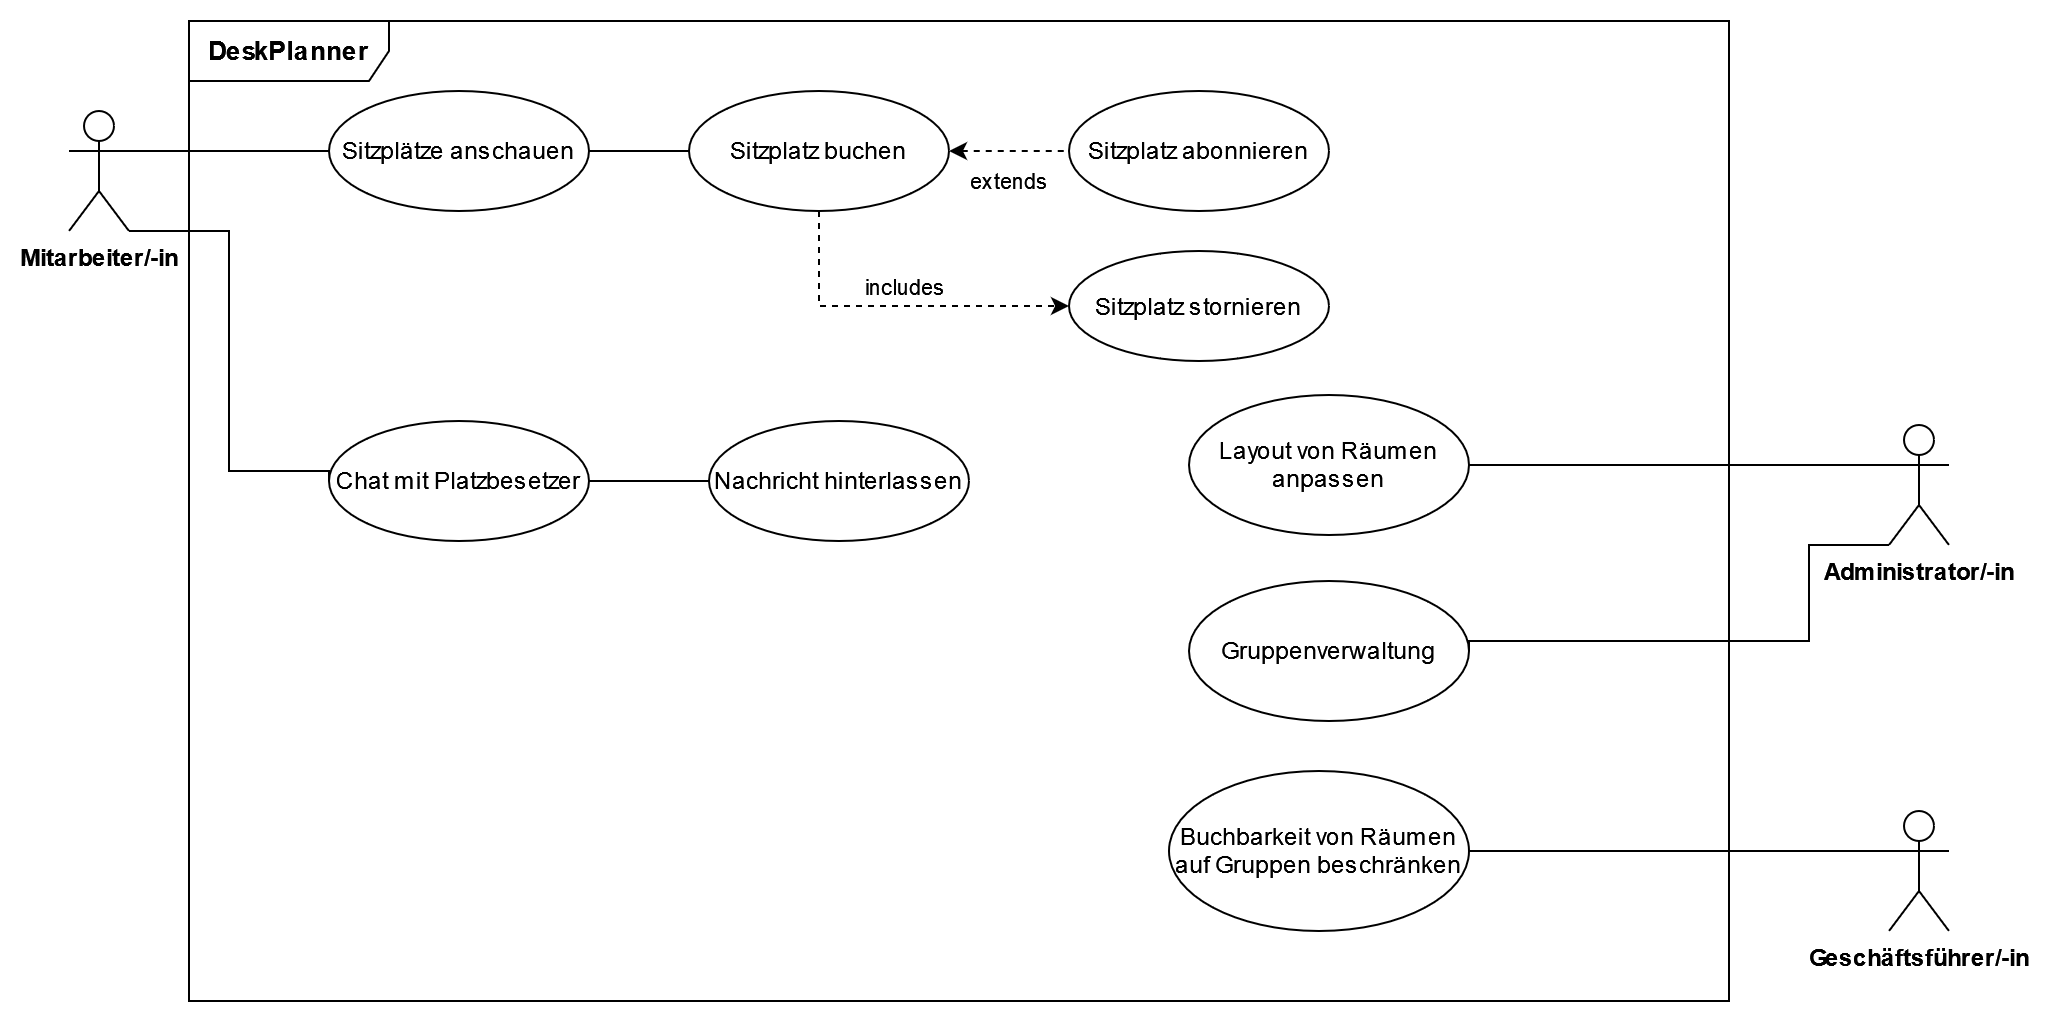
\includegraphics[width=0.8\textwidth]{UseCase_Diagram.png}
    \caption{Usecase-Diagramm}
    \label{fig:Usecase-Diagramm}
\end{figure}

\include{./tex_files/ui_entwürfe}
>>>>>>> e2fd2fd2e6af937f85cef4ac210cc9da5b931ec0

\chapter{Technisches Konzept}

\section{Verwendete Frameworks}

\begin{table}[!ht]
    \centering
    \resizebox{\textwidth}{!}{\begin{tabular}{|l|l|} 
    \hline
    \textbf{NestJS}                                                                       & \textbf{ExpressJS}                                                                    \\ 
    \hline
    \emph{NodeJS Framwork}                                                              & \emph{NodeJS Framework}                                                             \\ 
    \hline
    + Durch vorgegebene Struktur lässt sich  & - Projekt wird bei großer Projektgröße schnell                \\
    das Projekt eher strukturiert halten & unstrukturiert \\
    \hline
    + Durch die strukturierte Arbeitsweise                & - Durch die Freiheit bei Technologiewahl  \\
    gut für Teams geeignet &  eher für einzelne Developer besser \\
    \hline
    - weniger Freiheit bei Implementation                                        & + Mehr Freiheit bei der Implementation        \\
      & durch weniger Strukturvorgaben \\
    \hline
    - Aufgrund strengerer Strukturvorgaben                    & + Durch einfachen Aufbau leicht zu erlernen                                  \\
    schwerer zu lernen & \\ 
    \hline
    - relativ neue Technologie mit weniger Nutzern                               & + Viele Nutzer und dadurch auch viel                           \\
     & Dokumentation \\
    \hline
    \end{tabular}}
    \end{table}

NestJS war eine Vorgabe des Product Owners (IT Designers Gruppe) für die Entwicklung einer Back-End API. 
Es ist ein Framework das auf der JavaScript Umgebung NodeJS aufbaut und den Code in Module, Controller und Services aufteilt und somit eine klare Struktur zur Entwicklung vorgibt.\\
Aufgrund diesen strengen Strukturvorgaben, sind NestJS Anwendungen, im Vergleich mit bspw. ExpressJS, sehr gut skalierbar.

\begin{table}[!h]
    \centering
    \resizebox{\textwidth}{!}{\begin{tabular}{|l|l|}
    \hline
    \textbf{React}                                                                      & \textbf{Angular}                                                                    \\ 
    \hline
    \emph{JS Library}                                                             & \emph{JS Library}                                                           \\ 
    \hline
    + Vorbereitung für Praxissemester  & - Nicht sicher im Praxissemester verwendet                \\
    (Wird mind. 1 Teammitglied sicher  & \\
    verwenden) & \\
    \hline
    + Sehr einfaches erstellen von GUIs                & - Erstellen von Benutzeroberflächen etwas  \\
     &  komplizierter\\
    \hline
    - weniger strukturiert                                        & + Schon sehr ähnlich zu NestJS strukturiert        \\ 
    \hline
    + mehr Freiheit bei Implementation                    & - weniger Freiheit bei Implementation                                  \\ 
    \hline
    - aufgrund weniger Strukturvorgaben                               & + aufgrund der erzwungenen Struktur                           \\
    schwerer große Projekte sauber zu & ergeben sich auch bei großen \\
    halten & Projekten wenig Probleme \\
    \hline
    \end{tabular}}
    \end{table}

React ist sehr weit verbreitet und wird von vielen Firmen genutzt.
Daher wollte unser Team zunächst diese etwas weiter verbreitete Library lernen. 
Außerdem ist React im Vergleich zu Angular noch etwas einfacher zu lernen.
Daher fiel auch die Wahl auf React, trotz der sehr NestJS-ähnlichen Struktur die Angular bietet.


\begin{table}[!h]
    \centering
    \resizebox{\textwidth}{!}{\begin{tabular}{|l|l|}
    \hline
    \textbf{MongoDB}                                                                      & \textbf{MySQL}                                                                    \\ 
    \hline
    + No SQL Datenbank & - SQL Datenbank               \\ 
    \hline
    + Datenstrukturen sind näher an                 & - Datenstrukturen sind abstrakt,  \\
    tatsächlicher Implementation & nicht so nah an der Implementation \\
    \hline
    + Speichert Daten im JSON Format   & - Speichert Daten in Tabellen        \\
     $\rightarrow$ Struktur nah an Objekten & \\
    \hline
    - Für uns neue Technologie                   & + Schon bekannt aus vorherigen Semestern                                  \\ 
    \hline
    \end{tabular}}
    \end{table}

Auch MongoDB war eine Vorgabe des ProductOwners.
Im Vergleich zu “klassischen” Datenbanken wie MySQL halten Mongo Datenbanken ihre Daten nicht in Tabellen, sondern in JSON Files in einer Baumstruktur, d.h. MongoDB ist eine sog. NoSQL Datenbank. \\
Daher ist MongoDB im Vergleich zu bspw. MySQL Datenbanken schon von der Grundstruktur der Datenhaltung sehr nah an der tatsächlich in der Entwicklung genutzten Strukturen der Implementation und verlangt so weniger Abstraktion als eine SQL Datenbank.
\pagebreak
\section{Softwarearchitektur}

\begin{figure}[!h]
    \centering
    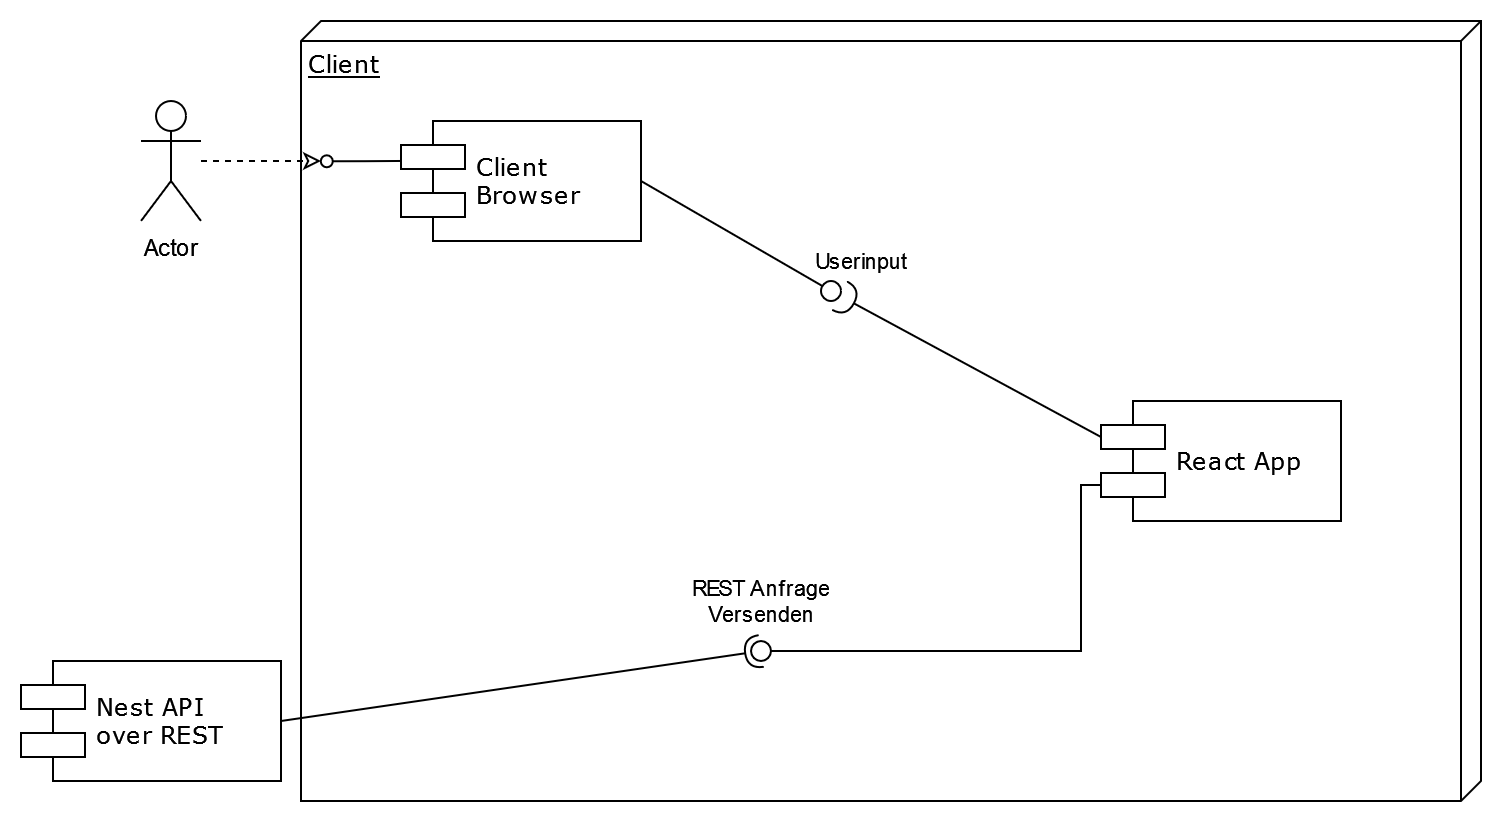
\includegraphics[width=0.8\textwidth]{./UML_Diagrams/ComponentDiagramClient.png}
    \caption{Component Diagram: Client}
    \label{fig:ComponentDiagramClient}
\end{figure}
In Abbildung 4.1 ist das Komponentendiagramm des Client zu sehen.
Dieses beschreibt die verwendeten Komponenten bei eingegangenem User Input.
Der Nutzer macht über den Web-Client eine Anfrage, wie beispielsweise der Aufruf der Web-Applikation oder die Anfrage auf einen bestimmten Raum.
Dadurch fordert der Client ein Interface über die React App, welche dann eine REST Anfrage an die Nest API schickt.
Im Normalfall sollte dann die REST Anfrage beantwortet werden und die React App kann mit den erhaltenen Informationen ein geeignetes User Interface zur Nutzung auf dem Client bereitstellen.

\begin{figure}[!h]
    \centering
    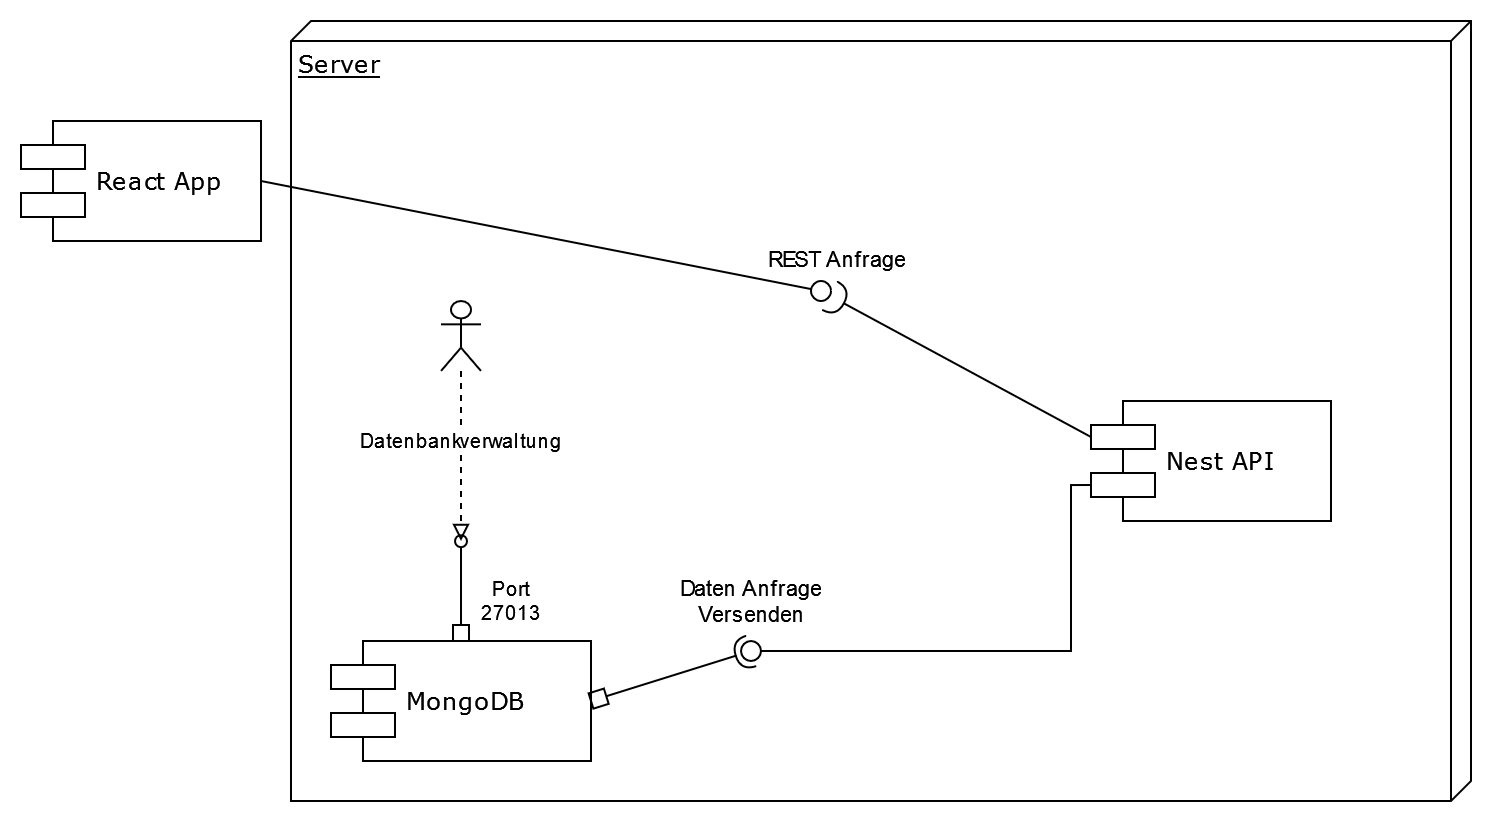
\includegraphics[width=0.8\textwidth]{./UML_Diagrams/ComponentDiagramServer.png}
    \caption{Component Diagram: Server}
    \label{fig:ComponentDiagramServer}
\end{figure}
In Abbildung 4.2 ist das Komponentendiagramm des Servers zu sehen.
Dieses beschreibt die verwendeten Komponenten bei eingegangener REST Anfrage.
Die React App stellt eine REST Anfrage an die NEST API, diese fordert dann die verlangten Informationen über ein Interface von der Mongo Datenbank.
Die MongoDB ist erreichbar über den Port 27013 durch den Datenbank-Administrator, dieser bearbeitet die Anfrage und sendet die gefordeten Daten über das Interface zurück an die Nest API.
Zu guter Letzt kann die Nest API dann die bereitgestellten Informationen über ein geeignetes Interface an die React App schicken, welche dadurch weitere Anfragen, wie mithilfe des Komponentendiagramm des Clients beschrieben wurde, beantworten kann.



\begin{figure}[!h]
    \centering
    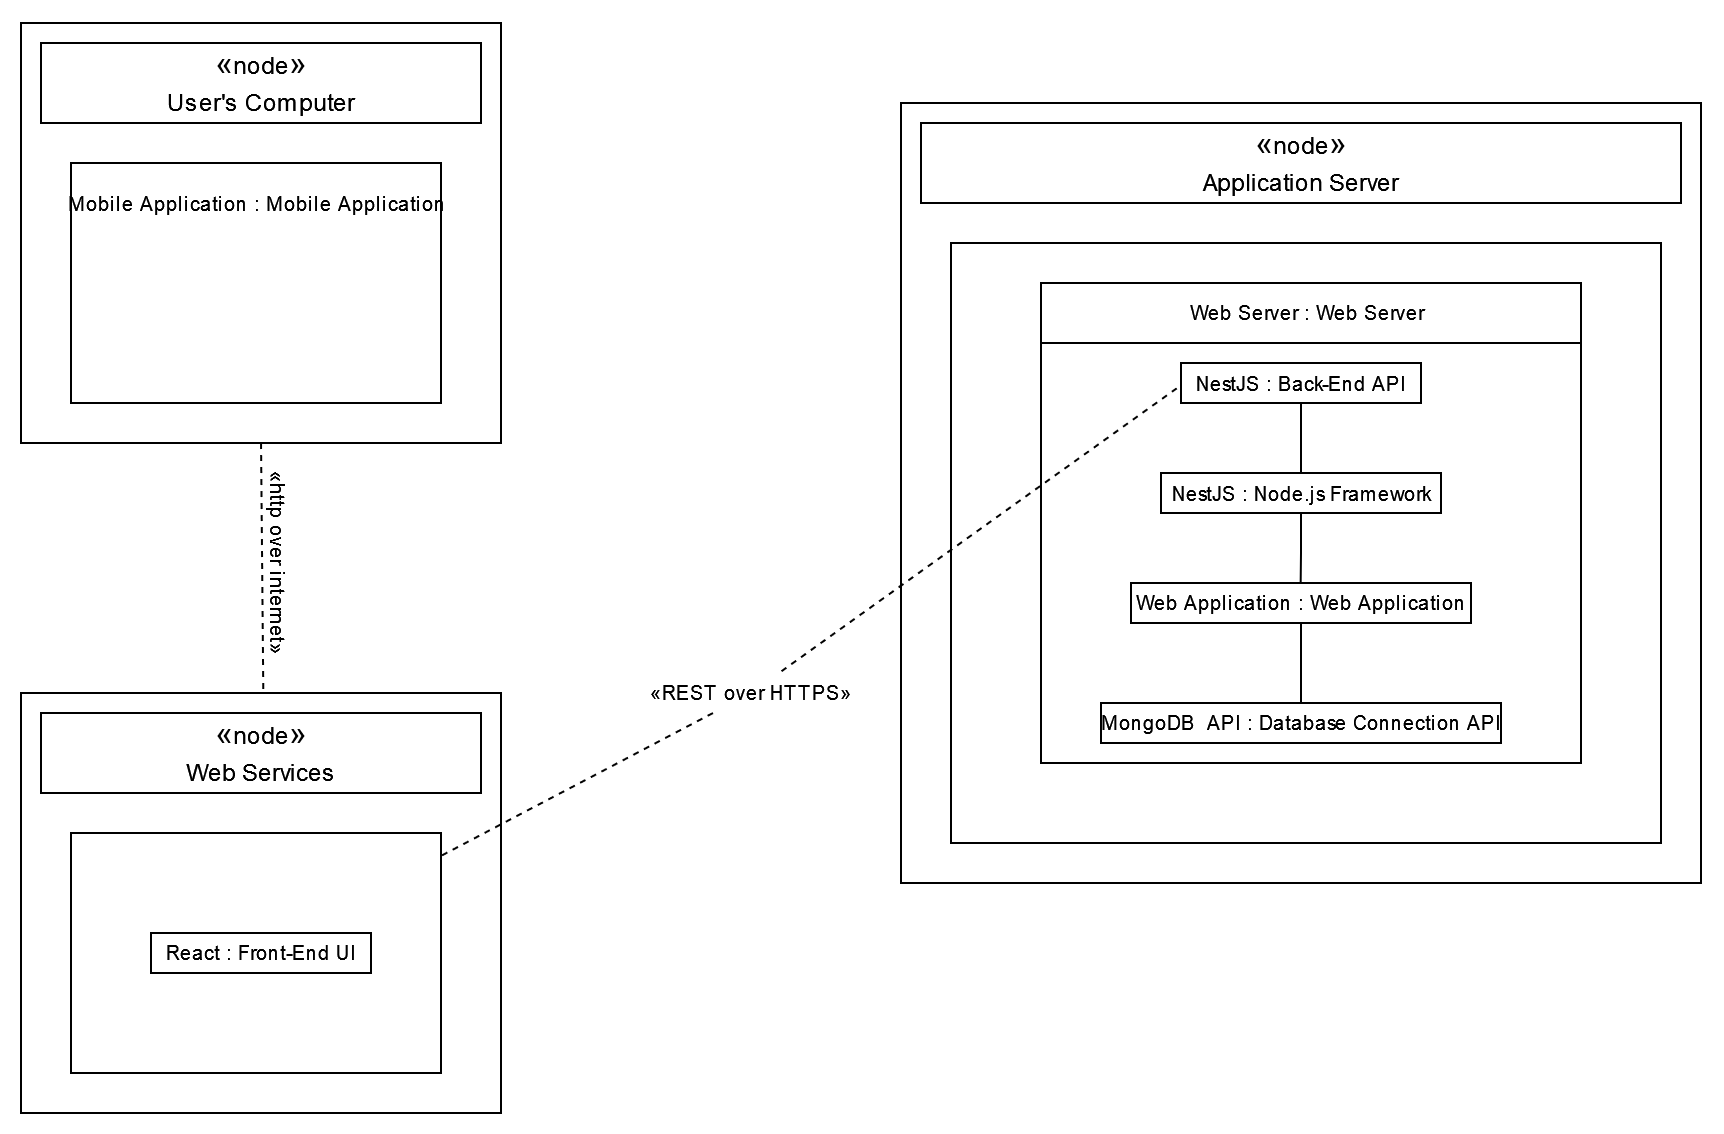
\includegraphics[width=0.8\textwidth]{./UML_Diagrams/Verteilungsdiagramm.png}
    \caption{Verteilungsdiagramm}
    \label{fig:Verteilungsdiagramm}
\end{figure}

Das in Abbildung 4.3 gezeigte Verteilungsdiagramm veranschaulicht, wie die Applikation im Browser des Nutzers über das React-Framework an das NestJS backend verbunden ist.
Der Nutzer sendet mithilfe der Benutzeroberflächen eine HTTP Anfrage an das React Front-End über das Internet, um zum Beispiel Informationen über Räume anzufordern.
Das React Front-End sendet die Anfrage des Nutzers mittels REST Anfrage über HTTPS an das NestJS Backend, damit dies an die Datenbank zugreifen kann.
Das NestJS Backend sendet die Anfrage an die Mongoose Datenbank und liefert die geforderten Informationen zurück.

\pagebreak
\section{Datenbanken}
\begin{figure}[!h]
    \centering
    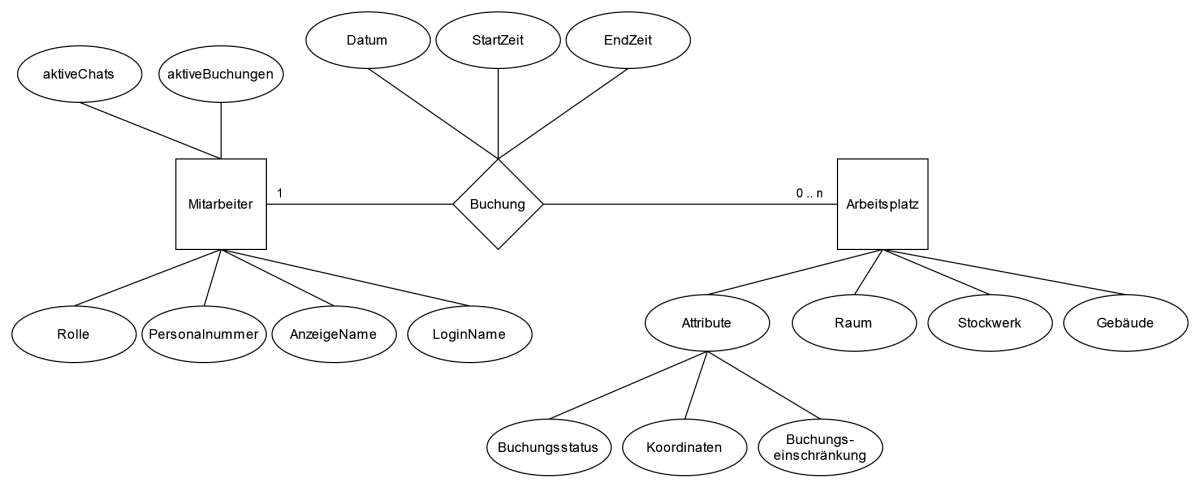
\includegraphics[width=1\textwidth]{./images/EntityRelationshipModel.png}
    \caption{Entity-Relationship-Modell}
    \label{fig:EntityRelationshipModel}
\end{figure}
Der Mitarbeiter hat eine Rolle. 
Unter Rollen versteht sich die Position im Betrieb, darunter zählt der Geschäftsleitung, der Administrator oder der Mitarbeiter.
Die Personalnummer, der AnzeigeName und der LoginName sind zusätzliche Attribute.
Das Attribut aktiveChats steht für die Mitarbeiterchats, aktivBuchungen symbolisiert die getätigten Buchungen.
Die Buchungen haben als Attribut Datum, Startzeit und EndZeit.
Der Arbeitsplatz hat die Attribute Buchungsstatus, Koordinaten, die Räumlichkeiten abbilden, Buchungseinschränkung. 
Zudem gibt es Raum, Stockwerk und Gebäude, die den gebuchten Ort beschreiben. 
Ein Mitarbeiter kann mehrere Arbeitsplätze zu verschiedenen Daten, an verschiedenen Örtlichkeiten gleichzeitig buchen. 


% Bibliography
% \bibliography{file.bibtex}
\bibliographystyle{plain}

% Ending of document
\end{document}
